\documentclass[letterpaper,12pt]{article}
\usepackage{tabularx} % extra features for tabular environment
\usepackage{amsmath}  % improve math presentation
\usepackage{graphicx} % takes care of graphic including machinery
\usepackage[margin=0.95in,letterpaper]{geometry} % decreases margins
\usepackage{cite} % takes care of citations
\usepackage[titletoc,title]{appendix} % takes care of appendices
\usepackage{listings} % code representation
\usepackage{pdflscape}
\usepackage{csquotes} % for quoting existing work
\usepackage{color} % defines colors for code listings
\usepackage{comment} % allows for block of comments
\usepackage[final]{hyperref} % adds hyper links inside the generated pdf file

% style code listings
\definecolor{codegreen}{rgb}{0,0.6,0}
\definecolor{codegray}{rgb}{0.5,0.5,0.5}
\definecolor{backcolour}{rgb}{0.95,0.95,0.92}
\lstdefinestyle{mystyle}{
    backgroundcolor=\color{backcolour},   
    commentstyle=\color{codegreen},
    keywordstyle=\color{blue},
    numberstyle=\tiny\color{codegray},
    basicstyle=\footnotesize,
    breakatwhitespace=false,         
    breaklines=true,                 
    captionpos=b,                    
    keepspaces=true,                 
    numbers=left,                    
    numbersep=5pt,                  
    showspaces=false,                
    showstringspaces=false,
    showtabs=false,                  
    tabsize=4
}
\lstset{style=mystyle}

\begin{document}

\title{CM30225 Parallel Computing\\Assessed Coursework Assignment 1}
\author{Adam Jaamour}
\date{19 November, 2018}
\maketitle


% ------------------------------------------ 1 - INTRODUCTION ------------------------------------------ 

\section{Introduction}

The objective of this assignment is to use low-level primitive parallelism constructs on a shared memory architecture and analyse how parallel problems scale on such an architectures using \textit{C} and \textit{pthreads} on Balena, a mid-sized cluster with 2720 cpu cores\cite{balena_notes}.\\

The background is a method called \textit{relaxation technique}, a solution to differential equations, which is achieved by having a square array of values and repeatedly replacing a value with the average of its four neighbours, excepting boundaries values which remain fixed. This process is repeated until all values settle down to within a given precision.


% ------------------------------------------ 2 - IMPLEMENTATION ------------------------------------------ 

\section{Implementation}

\subsection{Parallelism}
\label{sec:implementation_parallelism}

In this program, shared memory parallelism was implemented in C using POSIX threads \cite{posix_threads}. Amongst the multiple approaches to using \textit{pthreads} for parallelism that exist, one favouring efficiency and minimal overhead was chosen. This was achieved by first writing an efficient sequential version of the program, and then scaling it to parallel by using the least \textit{pthread} management possible, such as avoiding the use of barriers and focusing on mutexes to achieve a solution in parallel.\\

The solution uses two global arrays that can be accessed by all threads simultaneously: a square array of doubles holding the values to average, and a second array made up of mutexes only. After the threads' creation, each of them starts looping iteratively through the square array of double values. Whenever a thread accesses a value to read and update it, it locks access to that value as well as to its four neighbours that are used to calculate the new average. The locked values are only unlocked once their updated value has been written.\\

The thread locking a value in the array of doubles uses the mutex positioned in the same location in the second array of mutexes to lock the value being updated (and its four neighbour values). For example, if a thread is accessing the double value located at position $[i=4; j=6]$ in the first array, then it will use the mutex located at the same position in the second array of mutexes to lock the value. See Listing \ref{lst:loop_code} for the implementation in C.\\

\begin{lstlisting}[language=C, caption=Looping through the arrays (main.c), label={lst:loop_code}]
double **square_array;
pthread_mutex_t **mutex_array;

void* relaxation_runner(void* arg) {
    // ...
    for (i = 1; i < dim - 1; i++) {
    	for (j = 1; j < dim - 1; j++) {
    		// lock and retrieve current value to replace
    		pthread_mutex_lock(&mutex_array[i][j]);
    		double old_value = square_array[i][j];
    		// retrieve the 4 surrounding values needed to average
    		double v_left = square_array[i][j-1];
    		double v_right = square_array[i][j+1];
    		double v_up = square_array[i-1][j];
    		double v_down = square_array[i+1][j];
    		// calculate new value, replace the old value and unlock
    		double new_value = (v_left + v_right + v_up + v_down) / 4;
    		square_array[i][j] = new_value;
    		pthread_mutex_unlock(&mutex_array[i][j]);
    		// ...
    	}
    }
}
\end{lstlisting}

This solution can be pictured as a game of snake \cite{snake_game}, with the first thread representing the snake's head and the last thread representing its tail. The first thread iterates through the array starting at $[i=1; j=1]$, updating the value at this location, before moving on to $[i=1; j=2]$. As the first thread is moving through the array, the second thread and all the others will follow the same path as the first thread once they are scheduled. If they catch up with the first thread, they will have wait for it to unlock the value it is updating before accessing it, like a game of snake where the each body part follows the part in front of it once it moves.\\

This might cause a lot of overhead for very small array dimensions, but will cause less overhead as the arrays are larger in size. Indeed, arrays with dimensions of $5000\cdot5000$, equivalent to 25 million values in the array, can be solved in less than 10 minutes on Balena using a precision of $0.01$. See Section \ref{sec:analysis} for more information on the results of this implementation.

\subsection{Code}

\subsubsection{Structure}

The code was written following the C89 standard. It is divided in three source files to organize the code in logical sections:

\begin{itemize}
    \item main.c: The main code where the program starts executing. Contains the threaded function, \textit{relaxation\_runner}, that averages the array by iterating through it. It also contains all the global variables used throughout the program i.e. the program parameters such as array dimensions, precision to average to, number of threads to use and the initial array of double values.
    \item array\_helpers.c: This source file contains functions to allocate space to arrays, initialise them and populate them with values.
    \item print\_helpers.c: This source file hosts functions used to print data to the command line.
\end{itemize}

\subsubsection{Additional notes}

The function \textit{gettimeofday} from the \textit{sys/time.h} library \cite{c_systime} was used to calculate the time needed to find a solution. It started recording time before creating the threads and stopped right after all the threads stopped executing. See Listing \ref{lst:time_code} for the implementation of time.

\begin{lstlisting}[language=C, caption=Recording time (main.c), label={lst:time_code}]
#include <sys/time.h>
struct timeval time1, time2;

int main(int argc, char *argv[]) {
    // start recording time
	gettimeofday(&time1, NULL);
	// create threads
	for (i = 0; i < num_thr; i++) {
		pthread_create(&tids[i], &attr, relaxation_runner, &args[i]);
	}
	// wait until threads finish running
	for (i = 0; i < num_thr; i++) {
		pthread_join(tids[i], NULL);
	}
	// stop recording time
	gettimeofday(&time2, NULL); 
}
\end{lstlisting}

An important point to note is the effect of printing statements on the program's speed. Indeed, printing information on the command line using the \textit{printf} function considerably slows down the program, especially when these are located inside the threaded function's for loops. This means that \textit{printf} could sometimes be called millions of times in a single execution of the program, which distorted the final results. The solution was to use a global boolean as a condition to execute the calls to \textit{printf}, allowing for easy turning on/off print statements. 

\subsection{Balena}

The program needed to be run on Balena hundreds of times using different parameters, namely varying array sizes and number of threads, to gather relevant data. This meant that some automation was required to avoid executing each program one at a time manually.\\

The first automation process was the \textit{makefile}, which allowed for quick compilation of the three source files into \textit{.exe} executable files (See Appendix\ref{sec:makefile}). The dimension of the array would be specified in the \textit{main.c} source file before being compiled.\\

Next, a bash script was used to automate the submissions to Balena. It would submit 16 jobs at a time to Balena using the SLURM script (see Appendix \ref{sec:slurm}), each with a different number of threads passed as a command line argument (see Appendix \ref{sec:bash}). The first submission for a single array dimension would run on 1 to 16 threads (with increments of 1), and the second submission would run on 20 to 95 threads (with increments of 5).\\

Once the jobs finished executing on the cluster, they would be stored in directories named according on the parameters used. For example, jobs that were run to solve arrays dimensions of 1000 to a precision of 0.01 using 16 cores were stored in "dim1000\_\_cores16\_\_prec01". After all the resulting files were produced, they were exported to a plain text file where a regular expression was used to extract the solving durations for each program that ran with different parameters. These values were then pasted into an Excel spreadsheet where they were organised and plotted into graphs for analysis in Section \ref{sec:analysis}.\\

\subsection{Correctness Testing}

To ensure that the program was correctly solving the initial array, small parameters were used i.e. array dimension of 5, precision of 0.1 and array values ranging from 1 to 10. This allowed for writing down the process of solving the initial array on paper, and comparing the final array with the program output. The assumption that the program being correct for small arrays would be correct for larger arrays as well was made. When transitioning from sequential to parallel solving, the same initial array for the paper testing was used to check that the final array was correct after every update carried out on the code. Additionally, any warnings provided by GCC were fixed with the use of multiple flags such as \textit{Wall}, \textit{Wextra} and \textit{Wconversion}, ensuring that the C code itself was correct.


% ------------------------------------------ 3 - ANALYSIS ------------------------------------------ 

\section{Analysis}
\label{sec:analysis}

A total of 448 jobs were submitted to Balena to gather all the data needed to analyse the program (see Appendix \ref{sec:raw_data}). These jobs were run using the following parameters:
\begin{itemize}
    \item Ten different array dimensions, ranging from 5 to 5000, with random double values generated between 0 and 100. The array dimensions are organised in two parts: large arrays for dimensions of 500, 1000, 2500, 4500 and 5000, and small arrays for dimensions of 5, 10, 25, 50 and 100.
    \item Thirty-two different thread configurations, ranging from a single thread to 95.
    \item Two different numbers of core configurations: 16 and 4 cores.
    \item A precision of 0.01.
\end{itemize}

Plotting the raw output results, which represent the time needed to solve the array in seconds, does not provide much insight into the advantages of running the program in parallel rather than sequentially. Figure \ref{fig:time} tells us that larger arrays take more time to solve than smaller arrays, especially when the number of threads is small (approximately under 10). However, these large arrays seem to make the most of an increasing number of threads, allowing them to be solved faster as the number of threads increases, whereas small arrays do not gain speed from more threads. Indeed, looking at the raw data in Appendix \ref{sec:raw_data}, very small arrays of sizes 5, 10 and 25 actually slow down as the number of threads used rises.\\

\begin{figure}[h]
\centerline{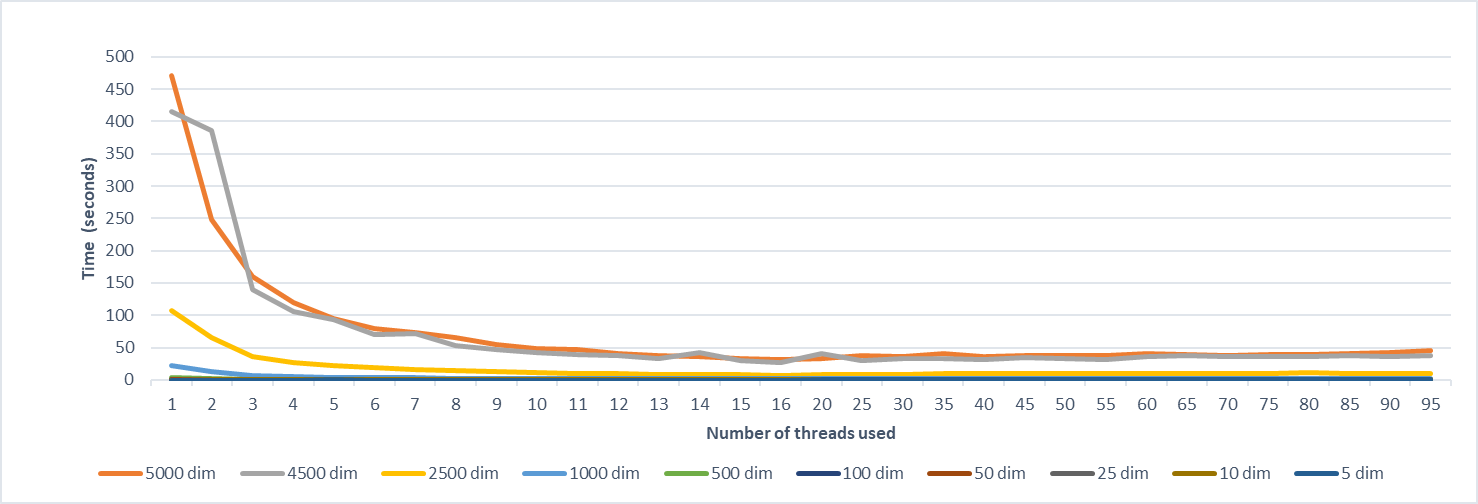
\includegraphics[width=\textwidth]{report/plots/time.png}}
\caption{\label{fig:time}Graph depicting the time needed to solve the array in seconds.}
\end{figure}

Solely analysing the time needed to solve the arrays does not provide enough insights to fully evaluate the gains of running a program in parallel. However, the time needed to solve the arrays in parallel can be directly compared with the time needed to solve the same arrays sequentially. This measure, known as the \textit{speedup}, is calculated as follows: $speedup = time_{sequential} / time_{parallel}$. Figure \ref{fig:speedup_big} illustrates how large arrays ranging from dimensions of 500 to 5000 benefit from speedups of 2.5 to 4.5. It is also very important to notice how the speedup increases in a linear fashion when running in parallel with 1 to 16 threads, but that as soon as more than 16 threads are used, the speedup flattens out and eventually starts slowly decreasing.\\

\begin{figure}[h]
\centerline{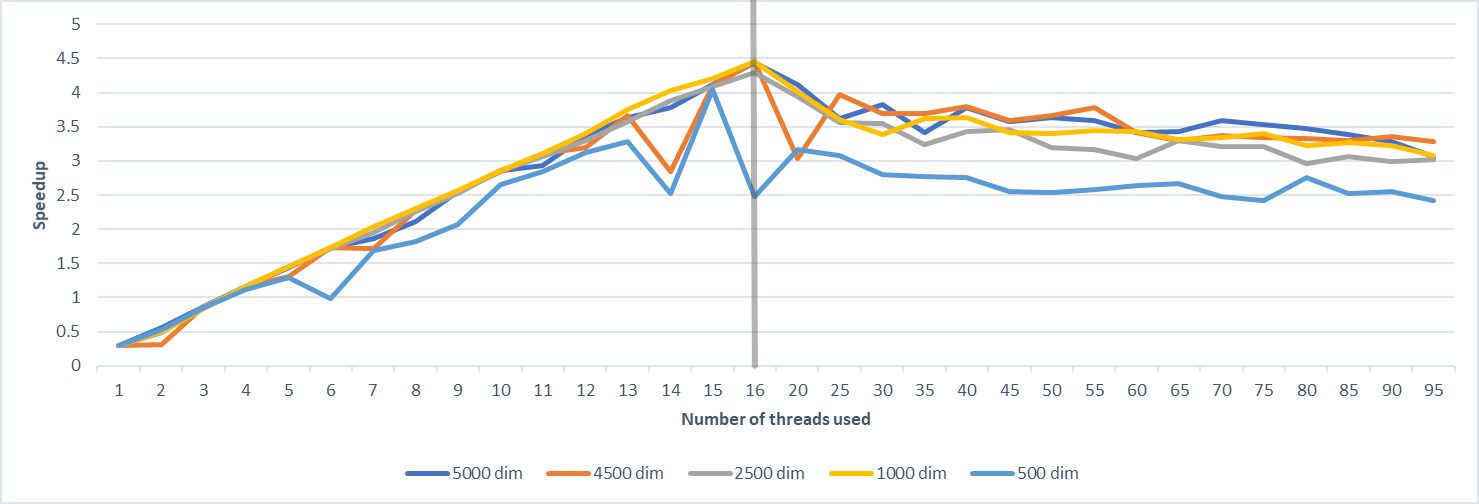
\includegraphics[width=\textwidth]{report/plots/speedup_big.png}}
\caption{\label{fig:speedup_big}Graph depicting the speedup gained for large-dimension arrays.}
\end{figure}

A hypothesis can be made regarding how Balena affects the speeds of the program running in parallel when more than 16 threads are being used. According the ``Notes on Balena'' available on the course's webpage \cite{balena_notes}, Balena has: 
\begin{displayquote}
``170 “standard” nodes of two Intel Xeon E5-2650v2 IvybridgeV2 CPUs, each having 8 cores, thus 16 symmetric shared memory cores on a node, giving us 2720 CPU cores.''
\end{displayquote} 
Each job submitted on Balena ran on a single node (see Appendix \ref{sec:slurm}, line 6), meaning 16 cores were available to the program every time it ran on the cluster. This can be an explanation as to why the program ran efficiently up until 16 threads with high speedups before starting to decrease in speed as more threads were used. It is therefore safe to assume that the hypothesis is true and that the operating system scheduled the threads efficiently when there were no more than 16. A reason for this could be that the OS scheduled each thread so that each thread fully used a single CPU to solve the array. As more threads than CPUs were created, the overhead of scheduling the threads across the 16 CPUs increased, thus causing the program to slow down considerably. This is also a reason as to why the highest speedup occurs when exactly 16 threads are in use.\\

When solving smaller arrays ranging from dimensions of 5 to 100, as represented in Figure \ref{fig:speedup_small}, the speedup is less significant than for larger arrays. As a matter of fact, the speedup is inferior to 1 for arrays under dimensions of 100, meaning that the sequential version of the program is quicker than the parallel one. This is mainly due to the fact that the small array size causes threads to often wait for each other as values are locked by the thread currently updating them (see Section \ref{sec:implementation_parallelism} for more information on the parallel implementation). Threads trying to access the same values occur less often for larger arrays than for smaller arrays, explaining the reason why the speedup is much higher for larger arrays (See Figure \ref{fig:speedup_big}) than for smaller arrays (See Figure \ref{fig:speedup_small}).\\

\begin{figure}[h]
\centerline{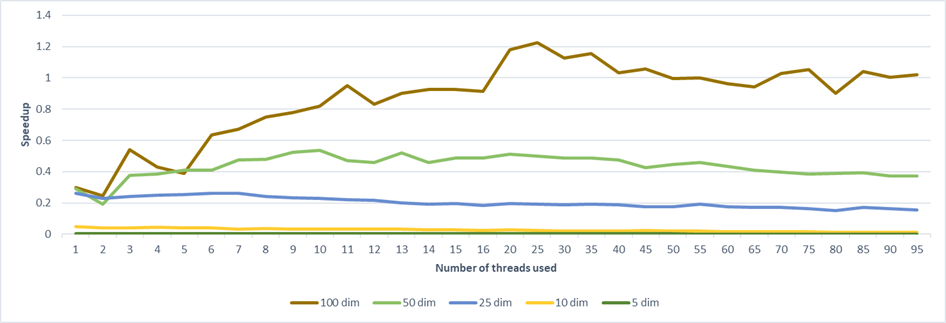
\includegraphics[width=\textwidth]{report/plots/speedup_small.png}}
\caption{\label{fig:speedup_small}Graph depicting the speedup gained for small-dimension arrays.}
\end{figure}

Another more detailed method of analysing the advantages (or disadvantages) of running a program in parallel rather than sequentially is by calculating the \textit{efficiency}. The efficiency can be calculated by using the speedup previously calculated with the number of threads used as follows: $efficiency = time_{sequential} / (p \cdot time_{parallel})$, where $p$ corresponds to the number of threads used.\\

Using the efficiency confirms the observations made from the speedup graphs. Indeed, the efficiency for large arrays resides around the 20\% to 30\% slice, as seen in Figure \ref{fig:efficiency_big}, meaning that approximately less than one third of processors' power is being used for the computation, with the rest being lost in overheads such as communication, printing or idling while waiting for array values to be unlocked. The same cutoff as in Figure \ref{fig:speedup_big} can be seen when \textit{number of threads used = 16}, where the efficiency considerably drops more than 16 threads are used, thus reinforcing the hypothesis made earlier about the 16 cores in a node being only efficiently used when there are 16 threads or less.\\

\begin{figure}[h]
\centerline{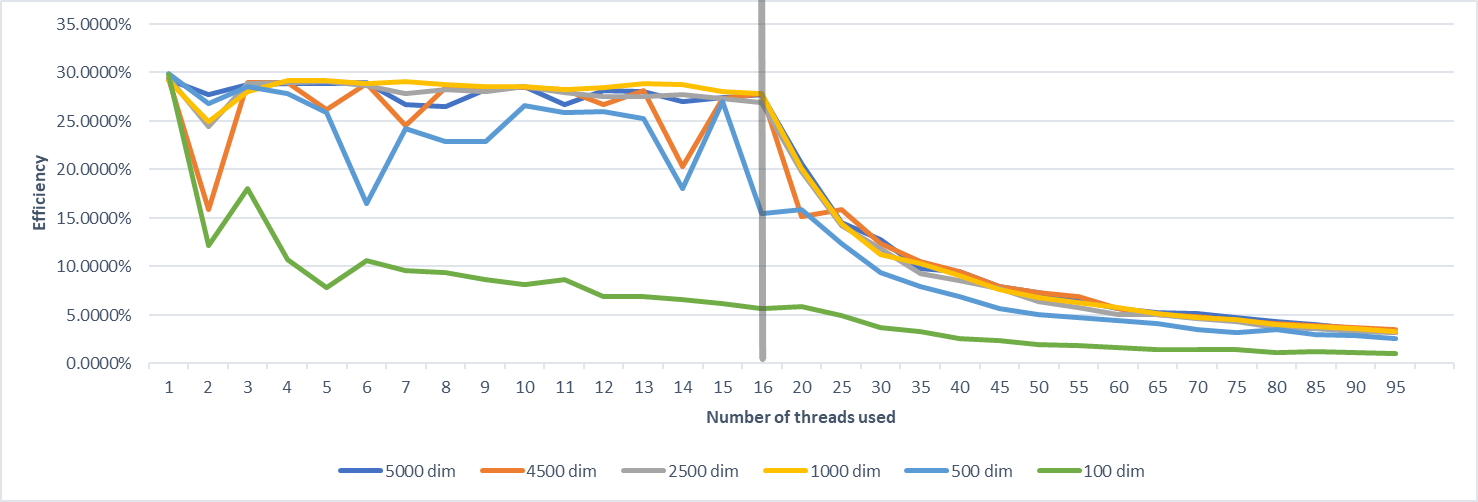
\includegraphics[width=\textwidth]{report/plots/efficiency_big.png}}
\caption{\label{fig:efficiency_big}Graph depicting the efficiency of running in parallel for large-dimension arrays.}
\end{figure}

Similarly to the speedup for smaller arrays, the efficiency is less important for small arrays than it is for large arrays as the efficiency quickly converges towards 0.001\% as more threads are used. Figure \ref{fig:efficiency_small} clearly portrays how inefficient parallelism is for small sized-problems as the program is the most efficient when running on a single thread. Running on four threads already makes the program three times less efficient than running on one thread.\\

\begin{figure}[h]
\centerline{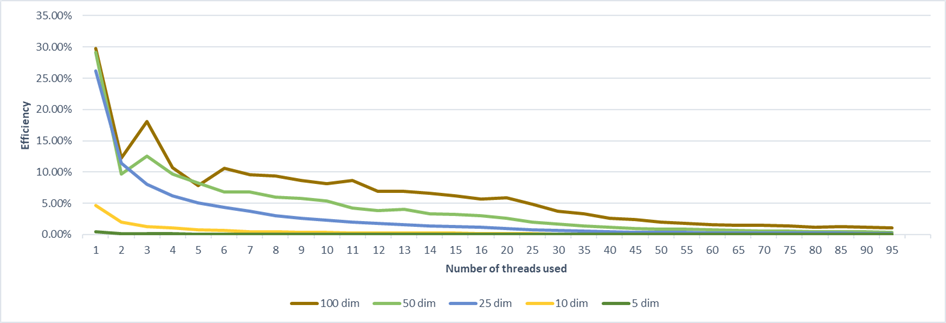
\includegraphics[width=\textwidth]{report/plots/efficiency_small.png}}
\caption{\label{fig:efficiency_small}Graph depicting the efficiency of running in parallel for small-dimension arrays.}
\end{figure}

It is important to note that during the data gathering phase, jobs using 4 cores instead of 16 were submitted to Balena. This was done by changing a line in the SLURM script from ``\textit{\#SBATCH --ntasks-per-node=16}'' to ``\textit{\#SBATCH --ntasks-per-node=4}''. The same test parameters were used for arrays of dimensions 100, 1000 and 2500, running on 1 to 95 threads with a precision of 0.01. However, the resulting data was near identical to the data produced when running on 16 cores, probably indicating that the jobs were not submitted correctly to run on 4 cores. Therefore, the results were not provided in this report as they too similar to the ones produced when running on 16 cores and would not provided any additional information.\\


% ------------------------------------------ 4 - CONCLUSION ------------------------------------------ 

\section{Conclusions}
There are many different ways of implementing parallelism in a program in a shared memory architecture. The analysis of the time, speedup and efficiency of running a program in parallel provided useful information regarding the scalability of such programs. Indeed, on the one hand, it is obvious that parallel programs scale well for large problems, whereas on the other hand this kind of solution does not suit small problems. \\

Another important point is that too much parallelism slows down the program considerably. All of the graphs in this report show that as more threads were used, the execution time rose and the speedup and efficiency diminished. Using too many parallel functions or constructs would have slowed down the program even more. For instance, if barriers were used to sync the threads between each other, an important amount of overhead would have been added in idling alone while the threads joined each other. Waiting threads are the main reason why some parallel implementations of program show poor performance.\\

With this particular implementation of parallelism, the number of CPUs available affected the number of threads that could be used efficiently. Another solution to solve this assignment with parallelism could have been to assign each thread specific locations of the array of values to solve, in which case the number of cores would have less affected the execution speed.\\

In conclusion, parallelism in code exists in multiple forms and will work more efficiently in different conditions for different problem sizes, there is no single solution to parallelism.


% ------------------------------------------ BIBLIOGRAPHY ------------------------------------------ 

\newpage
\bibliographystyle{unsrt}
\bibliography{bibliography.bib}


% ------------------------------------------ APPENDIX ------------------------------------------ 

\newpage
\begin{appendices}

\section{Makefile}
\label{sec:makefile}
\begin{lstlisting}[language=make]
CC			= gcc
CFLAGS		= -Wall -Wextra -Wconversion
LDFLAGS		= -pthread
OBJFILES	= main.o array_helpers.o print_helpers.o
TARGET		= relaxation

all: $(TARGET)

$(TARGET): $(OBJFILES)
	$(CC) $(CFLAGS) -o $(TARGET) $(OBJFILES) $(LDFLAGS)
	
clean:
	rm -rf $(OBJFILES) $(TARGET) *~
\end{lstlisting}

\section{SLURM script}
\label{sec:slurm}

\begin{lstlisting}[language=bash]
#!/bin/bash
#SBATCH --account=cm30225
#SBATCH --partition=teaching
#SBATCH --job-name=aj645_cw1
#SBATCH --output=relaxation.%j.out
#SBATCH --nodes=1
#SBATCH --ntasks-per-node=16
#SBATCH --mail-type=END
#SBATCH --mail-user=aj645@bath.ac.uk
./relaxation $1
\end{lstlisting}

\section{Bash Submission Script}
\label{sec:bash}

\begin{lstlisting}[language=bash]
#!/bin/sh
for i in 0 1 2 3 4 5 6 7 8 9 10 11 12 13 14 15
do
    n=`expr $i \* 1 + 1`  # increment 1 by 1, starting from 1
    # OR
	n=`expr $i \* 5 + 20` # increment 5 by 5, starting from 20
    sbatch job.slurm $n A
done

\end{lstlisting}

\newpage
\section{Raw Data}
\label{sec:raw_data}

\begin{table}[ht]
\centering
\begin{tabular}{|l|l|}
\hline
\textbf{threads}  & \textbf{time} \\ \hline
\textbf{5000 dim} & 137.4530            \\ \hline
\textbf{4500 dim} & 122.0865            \\ \hline
\textbf{2500 dim} & 31.7127             \\ \hline
\textbf{1000 dim} & 6.2657              \\ \hline
\textbf{500 dim}  & 1.1366              \\ \hline
\textbf{100 dim}  & 0.0323              \\ \hline
\textbf{50 dim}   & 0.006891            \\ \hline
\textbf{25 dim}   & 0.001572            \\ \hline
\textbf{10 dim}   & 0.000028            \\ \hline
\textbf{5 dim}    & 0.000002            \\ \hline
\end{tabular}
\caption{Data representing sequential solve time in seconds for square arrays between dimensions of 5 and 5000 running on 1 to 95 threads with a precision of 0.01 on 16 cores.}
\end{table}

\begin{landscape}
\begin{table}[ht]
\begin{tabular}{|l|l|l|l|l|l|l|l|l|l|l|}
\hline
\textbf{threads} & \textbf{5000 dim} & \textbf{4500 dim} & \textbf{2500 dim} & \textbf{1000 dim} & \textbf{500 dim} & \textbf{100 dim} & \textbf{50 dim} & \textbf{25 dim} & \textbf{10 dim} & \textbf{5 dim} \\ \hline
\textbf{1}       & 470.3395          & 415.8205          & 107.4633          & 21.4840           & 3.7975           & 0.1087           & 0.0236          & 0.0060          & 0.0006          & 0.0005         \\ \hline
\textbf{2}       & 247.9525          & 385.3578          & 64.8323           & 12.5507           & 2.1167           & 0.1326           & 0.0356          & 0.0069          & 0.0007          & 0.0005         \\ \hline
\textbf{3}       & 159.2870          & 140.5821          & 36.5744           & 7.4518            & 1.3275           & 0.0597           & 0.0183          & 0.0065          & 0.0007          & 0.0005         \\ \hline
\textbf{4}       & 119.0060          & 105.2247          & 27.3287           & 5.3765            & 1.0225           & 0.0755           & 0.0179          & 0.0063          & 0.0007          & 0.0005         \\ \hline
\textbf{5}       & 95.3892           & 93.0949           & 21.8008           & 4.2978            & 0.8770           & 0.0831           & 0.0168          & 0.0062          & 0.0007          & 0.0007         \\ \hline
\textbf{6}       & 79.1536           & 70.4467           & 18.4627           & 3.6224            & 1.1470           & 0.0509           & 0.0168          & 0.0060          & 0.0007          & 0.0006         \\ \hline
\textbf{7}       & 73.4592           & 71.0275           & 16.2992           & 3.0750            & 0.6709           & 0.0482           & 0.0145          & 0.0060          & 0.0009          & 0.0006         \\ \hline
\textbf{8}       & 64.8927           & 53.6704           & 14.0181           & 2.7262            & 0.6223           & 0.0430           & 0.0143          & 0.0065          & 0.0008          & 0.0005         \\ \hline
\textbf{9}       & 54.0010           & 47.6978           & 12.5571           & 2.4373            & 0.5512           & 0.0415           & 0.0132          & 0.0067          & 0.0008          & 0.0006         \\ \hline
\textbf{10}      & 48.1013           & 42.9142           & 11.0921           & 2.1959            & 0.4280           & 0.0395           & 0.0128          & 0.0068          & 0.0009          & 0.0006         \\ \hline
\textbf{11}      & 46.8245           & 39.3487           & 10.3370           & 2.0167            & 0.3995           & 0.0341           & 0.0147          & 0.0071          & 0.0009          & 0.0006         \\ \hline
\textbf{12}      & 40.7194           & 38.1313           & 9.6005            & 1.8381            & 0.3643           & 0.0388           & 0.0150          & 0.0073          & 0.0009          & 0.0006         \\ \hline
\textbf{13}      & 37.7367           & 33.3627           & 8.8492            & 1.6679            & 0.3466           & 0.0359           & 0.0133          & 0.0079          & 0.0008          & 0.0005         \\ \hline
\textbf{14}      & 36.3150           & 42.9005           & 8.1587            & 1.5563            & 0.4498           & 0.0349           & 0.0151          & 0.0082          & 0.0010          & 0.0006         \\ \hline
\textbf{15}      & 33.3729           & 29.7582           & 7.7418            & 1.4913            & 0.2807           & 0.0349           & 0.0141          & 0.0080          & 0.0010          & 0.0006         \\ \hline
\textbf{16}      & 30.9489           & 27.4219           & 7.3812            & 1.4084            & 0.4586           & 0.0355           & 0.0142          & 0.0086          & 0.0013          & 0.0005         \\ \hline
\textbf{20}      & 33.4148           & 40.1902           & 8.0306            & 1.5626            & 0.3585           & 0.0274           & 0.0135          & 0.0081          & 0.0011          & 0.0007         \\ \hline
\textbf{25}      & 37.8875           & 30.6813           & 8.9041            & 1.7404            & 0.3684           & 0.0264           & 0.0138          & 0.0082          & 0.0012          & 0.0008         \\ \hline
\textbf{30}      & 35.9892           & 32.9891           & 8.9498            & 1.8510            & 0.4053           & 0.0287           & 0.0141          & 0.0083          & 0.0015          & 0.0009         \\ \hline
\textbf{35}      & 40.2581           & 33.0721           & 9.7879            & 1.7312            & 0.4092           & 0.0280           & 0.0142          & 0.0082          & 0.0015          & 0.0010         \\ \hline
\textbf{40}      & 36.3527           & 32.0929           & 9.2289            & 1.7230            & 0.4127           & 0.0313           & 0.0145          & 0.0083          & 0.0014          & 0.0012         \\ \hline
\textbf{45}      & 38.3879           & 34.0515           & 9.1541            & 1.8335            & 0.4455           & 0.0306           & 0.0161          & 0.0089          & 0.0012          & 0.0012         \\ \hline
\textbf{50}      & 37.7875           & 33.3383           & 9.9141            & 1.8446            & 0.4472           & 0.0325           & 0.0155          & 0.0090          & 0.0014          & 0.0014         \\ \hline
\textbf{55}      & 38.2147           & 32.2409           & 10.0319           & 1.8201            & 0.4391           & 0.0324           & 0.0150          & 0.0081          & 0.0014          & 0.0015         \\ \hline
\textbf{60}      & 40.2797           & 35.7707           & 10.4536           & 1.8236            & 0.4312           & 0.0336           & 0.0158          & 0.0090          & 0.0016          & 0.0017         \\ \hline
\textbf{65}      & 40.0038           & 37.0199           & 9.5981            & 1.8868            & 0.4254           & 0.0344           & 0.0168          & 0.0091          & 0.0017          & 0.0017         \\ \hline
\textbf{70}      & 38.3269           & 36.1915           & 9.8800            & 1.8773            & 0.4576           & 0.0314           & 0.0174          & 0.0091          & 0.0019          & 0.0017         \\ \hline
\textbf{75}      & 38.9164           & 36.5719           & 9.8933            & 1.8445            & 0.4703           & 0.0307           & 0.0180          & 0.0096          & 0.0019          & 0.0021         \\ \hline
\textbf{80}      & 39.5962           & 36.6115           & 10.7171           & 1.9424            & 0.4118           & 0.0358           & 0.0178          & 0.0103          & 0.0021          & 0.0022         \\ \hline
\textbf{85}      & 40.4971           & 37.0459           & 10.3616           & 1.9145            & 0.4498           & 0.0310           & 0.0176          & 0.0092          & 0.0022          & 0.0022         \\ \hline
\textbf{90}      & 41.8654           & 36.3042           & 10.6075           & 1.9399            & 0.4455           & 0.0322           & 0.0184          & 0.0097          & 0.0024          & 0.0023         \\ \hline
\textbf{95}      & 44.8397           & 37.1102           & 10.4856           & 2.0313            & 0.4684           & 0.0317           & 0.0184          & 0.0100          & 0.0024          & 0.0025         \\ \hline
\end{tabular}
\caption{Data representing parallel solve time in seconds for square arrays between dimensions of 5 to 5000 running on 1 to 95 threads with a precision of 0.01on 16 cores.}
\end{table}
\begin{table}[ht]
\centering
\begin{tabular}{|l|l|l|l|l|l|l|l|l|l|l|}
\hline
\textbf{threads} & \textbf{5000 dim} & \textbf{4500 dim} & \textbf{2500 dim} & \textbf{1000 dim} & \textbf{500 dim} & \textbf{100 dim} & \textbf{50 dim} & \textbf{25 dim} & \textbf{10 dim} & \textbf{5 dim} \\ \hline
\textbf{1}       & 0.2922            & 0.2936            & 0.2951            & 0.2916            & 0.2993           & 0.2975           & 0.2920          & 0.2614          & 0.0470          & 0.0041         \\ \hline
\textbf{2}       & 0.5544            & 0.3168            & 0.4892            & 0.4992            & 0.5370           & 0.2439           & 0.1936          & 0.2286          & 0.0387          & 0.0038         \\ \hline
\textbf{3}       & 0.8629            & 0.8684            & 0.8671            & 0.8408            & 0.8562           & 0.5415           & 0.3756          & 0.2415          & 0.0394          & 0.0041         \\ \hline
\textbf{4}       & 1.1550            & 1.1602            & 1.1604            & 1.1654            & 1.1115           & 0.4286           & 0.3855          & 0.2479          & 0.0427          & 0.0042         \\ \hline
\textbf{5}       & 1.4410            & 1.3114            & 1.4547            & 1.4579            & 1.2960           & 0.3891           & 0.4112          & 0.2545          & 0.0394          & 0.0030         \\ \hline
\textbf{6}       & 1.7365            & 1.7330            & 1.7177            & 1.7297            & 0.9909           & 0.6356           & 0.4090          & 0.2604          & 0.0398          & 0.0036         \\ \hline
\textbf{7}       & 1.8711            & 1.7189            & 1.9457            & 2.0376            & 1.6941           & 0.6706           & 0.4744          & 0.2626          & 0.0313          & 0.0036         \\ \hline
\textbf{8}       & 2.1182            & 2.2747            & 2.2623            & 2.2983            & 1.8266           & 0.7516           & 0.4810          & 0.2427          & 0.0358          & 0.0037         \\ \hline
\textbf{9}       & 2.5454            & 2.5596            & 2.5255            & 2.5708            & 2.0621           & 0.7788           & 0.5240          & 0.2346          & 0.0336          & 0.0032         \\ \hline
\textbf{10}      & 2.8576            & 2.8449            & 2.8590            & 2.8534            & 2.6554           & 0.8182           & 0.5385          & 0.2307          & 0.0316          & 0.0035         \\ \hline
\textbf{11}      & 2.9355            & 3.1027            & 3.0679            & 3.1069            & 2.8449           & 0.9487           & 0.4697          & 0.2217          & 0.0305          & 0.0034         \\ \hline
\textbf{12}      & 3.3756            & 3.2017            & 3.3032            & 3.4089            & 3.1196           & 0.8336           & 0.4605          & 0.2156          & 0.0314          & 0.0036         \\ \hline
\textbf{13}      & 3.6424            & 3.6594            & 3.5837            & 3.7567            & 3.2797           & 0.9019           & 0.5200          & 0.1992          & 0.0334          & 0.0038         \\ \hline
\textbf{14}      & 3.7850            & 2.8458            & 3.8870            & 4.0261            & 2.5269           & 0.9275           & 0.4571          & 0.1906          & 0.0287          & 0.0033         \\ \hline
\textbf{15}      & 4.1187            & 4.1026            & 4.0963            & 4.2016            & 4.0495           & 0.9256           & 0.4881          & 0.1972          & 0.0286          & 0.0032         \\ \hline
\textbf{16}      & 4.4413            & 4.4522            & 4.2964            & 4.4488            & 2.4783           & 0.9121           & 0.4860          & 0.1825          & 0.0220          & 0.0036         \\ \hline
\textbf{20}      & 4.1135            & 3.0377            & 3.9490            & 4.0097            & 3.1708           & 1.1806           & 0.5102          & 0.1946          & 0.0263          & 0.0027         \\ \hline
\textbf{25}      & 3.6279            & 3.9792            & 3.5616            & 3.6002            & 3.0849           & 1.2242           & 0.4980          & 0.1909          & 0.0231          & 0.0025         \\ \hline
\textbf{30}      & 3.8193            & 3.7008            & 3.5434            & 3.3851            & 2.8040           & 1.1264           & 0.4883          & 0.1894          & 0.0187          & 0.0021         \\ \hline
\textbf{35}      & 3.4143            & 3.6915            & 3.2400            & 3.6192            & 2.7779           & 1.1539           & 0.4854          & 0.1908          & 0.0190          & 0.0021         \\ \hline
\textbf{40}      & 3.7811            & 3.8042            & 3.4363            & 3.6365            & 2.7540           & 1.0341           & 0.4747          & 0.1888          & 0.0203          & 0.0017         \\ \hline
\textbf{45}      & 3.5806            & 3.5854            & 3.4643            & 3.4173            & 2.5514           & 1.0578           & 0.4269          & 0.1763          & 0.0226          & 0.0016         \\ \hline
\textbf{50}      & 3.6375            & 3.6621            & 3.1988            & 3.3968            & 2.5414           & 0.9952           & 0.4447          & 0.1753          & 0.0206          & 0.0015         \\ \hline
\textbf{55}      & 3.5969            & 3.7867            & 3.1612            & 3.4426            & 2.5887           & 0.9992           & 0.4592          & 0.1936          & 0.0200          & 0.0013         \\ \hline
\textbf{60}      & 3.4125            & 3.4130            & 3.0337            & 3.4358            & 2.6358           & 0.9612           & 0.4349          & 0.1741          & 0.0178          & 0.0012         \\ \hline
\textbf{65}      & 3.4360            & 3.2979            & 3.3041            & 3.3208            & 2.6719           & 0.9409           & 0.4093          & 0.1729          & 0.0164          & 0.0012         \\ \hline
\textbf{70}      & 3.5863            & 3.3733            & 3.2098            & 3.3376            & 2.4838           & 1.0299           & 0.3952          & 0.1728          & 0.0146          & 0.0012         \\ \hline
\textbf{75}      & 3.5320            & 3.3383            & 3.2055            & 3.3970            & 2.4167           & 1.0518           & 0.3829          & 0.1636          & 0.0146          & 0.0010         \\ \hline
\textbf{80}      & 3.4714            & 3.3346            & 2.9591            & 3.2258            & 2.7600           & 0.9022           & 0.3873          & 0.1525          & 0.0131          & 0.0009         \\ \hline
\textbf{85}      & 3.3941            & 3.2955            & 3.0606            & 3.2727            & 2.5270           & 1.0425           & 0.3920          & 0.1715          & 0.0127          & 0.0009         \\ \hline
\textbf{90}      & 3.2832            & 3.3629            & 2.9897            & 3.2300            & 2.5512           & 1.0053           & 0.3737          & 0.1614          & 0.0119          & 0.0009         \\ \hline
\textbf{95}      & 3.0654            & 3.2898            & 3.0244            & 3.0846            & 2.4267           & 1.0190           & 0.3741          & 0.1565          & 0.0115          & 0.0008         \\ \hline
\end{tabular}
\caption{Data representing parallel speedup for square arrays between dimensions of 5 to 5000 running on 1 to 95 threads with a precision of 0.01 on 16 cores.}
\end{table}
\begin{table}[ht]
\centering
\begin{tabular}{|l|l|l|l|l|l|l|l|l|l|l|}
\hline
\textbf{threads} & \textbf{5000 dim} & \textbf{4500 dim} & \textbf{2500 dim} & \textbf{1000 dim} & \textbf{500 dim} & \textbf{100 dim} & \textbf{50 dim} & \textbf{25 dim} & \textbf{10 dim} & \textbf{5 dim} \\ \hline
\textbf{1}       & 29.224\%          & 29.360\%          & 29.510\%          & 29.165\%          & 29.930\%         & 29.746\%         & 29.195\%        & 26.139\%        & 4.698\%         & 0.410\%        \\ \hline
\textbf{2}       & 27.718\%          & 15.841\%          & 24.458\%          & 24.962\%          & 26.848\%         & 12.194\%         & 9.679\%         & 11.428\%        & 1.936\%         & 0.188\%        \\ \hline
\textbf{3}       & 28.764\%          & 28.948\%          & 28.902\%          & 28.028\%          & 28.539\%         & 18.050\%         & 12.519\%        & 8.049\%         & 1.313\%         & 0.136\%        \\ \hline
\textbf{4}       & 28.875\%          & 29.006\%          & 29.010\%          & 29.135\%          & 27.788\%         & 10.714\%         & 9.638\%         & 6.198\%         & 1.069\%         & 0.105\%        \\ \hline
\textbf{5}       & 28.819\%          & 26.228\%          & 29.093\%          & 29.158\%          & 25.919\%         & 7.782\%          & 8.224\%         & 5.090\%         & 0.789\%         & 0.059\%        \\ \hline
\textbf{6}       & 28.942\%          & 28.884\%          & 28.628\%          & 28.828\%          & 16.516\%         & 10.593\%         & 6.817\%         & 4.339\%         & 0.663\%         & 0.059\%        \\ \hline
\textbf{7}       & 26.731\%          & 24.555\%          & 27.795\%          & 29.109\%          & 24.201\%         & 9.580\%          & 6.777\%         & 3.751\%         & 0.447\%         & 0.052\%        \\ \hline
\textbf{8}       & 26.477\%          & 28.434\%          & 28.278\%          & 28.729\%          & 22.832\%         & 9.394\%          & 6.013\%         & 3.034\%         & 0.447\%         & 0.047\%        \\ \hline
\textbf{9}       & 28.282\%          & 28.440\%          & 28.061\%          & 28.565\%          & 22.912\%         & 8.653\%          & 5.823\%         & 2.606\%         & 0.373\%         & 0.035\%        \\ \hline
\textbf{10}      & 28.576\%          & 28.449\%          & 28.590\%          & 28.534\%          & 26.554\%         & 8.182\%          & 5.385\%         & 2.307\%         & 0.316\%         & 0.035\%        \\ \hline
\textbf{11}      & 26.686\%          & 28.206\%          & 27.890\%          & 28.244\%          & 25.863\%         & 8.624\%          & 4.270\%         & 2.015\%         & 0.277\%         & 0.031\%        \\ \hline
\textbf{12}      & 28.130\%          & 26.681\%          & 27.527\%          & 28.407\%          & 25.997\%         & 6.946\%          & 3.838\%         & 1.797\%         & 0.262\%         & 0.030\%        \\ \hline
\textbf{13}      & 28.019\%          & 28.149\%          & 27.567\%          & 28.897\%          & 25.229\%         & 6.938\%          & 4.000\%         & 1.532\%         & 0.257\%         & 0.029\%        \\ \hline
\textbf{14}      & 27.036\%          & 20.327\%          & 27.764\%          & 28.758\%          & 18.050\%         & 6.625\%          & 3.265\%         & 1.361\%         & 0.205\%         & 0.023\%        \\ \hline
\textbf{15}      & 27.458\%          & 27.351\%          & 27.309\%          & 28.010\%          & 26.996\%         & 6.170\%          & 3.254\%         & 1.315\%         & 0.191\%         & 0.022\%        \\ \hline
\textbf{16}      & 27.758\%          & 27.826\%          & 26.853\%          & 27.805\%          & 15.489\%         & 5.701\%          & 3.038\%         & 1.141\%         & 0.138\%         & 0.023\%        \\ \hline
\textbf{20}      & 20.568\%          & 15.189\%          & 19.745\%          & 20.049\%          & 15.854\%         & 5.903\%          & 2.551\%         & 0.973\%         & 0.132\%         & 0.013\%        \\ \hline
\textbf{25}      & 14.512\%          & 15.917\%          & 14.246\%          & 14.401\%          & 12.340\%         & 4.897\%          & 1.992\%         & 0.764\%         & 0.092\%         & 0.010\%        \\ \hline
\textbf{30}      & 12.731\%          & 12.336\%          & 11.811\%          & 11.284\%          & 9.347\%          & 3.755\%          & 1.628\%         & 0.631\%         & 0.062\%         & 0.007\%        \\ \hline
\textbf{35}      & 9.755\%           & 10.547\%          & 9.257\%           & 10.341\%          & 7.937\%          & 3.297\%          & 1.387\%         & 0.545\%         & 0.054\%         & 0.006\%        \\ \hline
\textbf{40}      & 9.453\%           & 9.510\%           & 8.591\%           & 9.091\%           & 6.885\%          & 2.585\%          & 1.187\%         & 0.472\%         & 0.051\%         & 0.004\%        \\ \hline
\textbf{45}      & 7.957\%           & 7.967\%           & 7.699\%           & 7.594\%           & 5.670\%          & 2.351\%          & 0.949\%         & 0.392\%         & 0.050\%         & 0.004\%        \\ \hline
\textbf{50}      & 7.275\%           & 7.324\%           & 6.398\%           & 6.794\%           & 5.083\%          & 1.990\%          & 0.889\%         & 0.351\%         & 0.041\%         & 0.003\%        \\ \hline
\textbf{55}      & 6.540\%           & 6.885\%           & 5.748\%           & 6.259\%           & 4.707\%          & 1.817\%          & 0.835\%         & 0.352\%         & 0.036\%         & 0.002\%        \\ \hline
\textbf{60}      & 5.687\%           & 5.688\%           & 5.056\%           & 5.726\%           & 4.393\%          & 1.602\%          & 0.725\%         & 0.290\%         & 0.030\%         & 0.002\%        \\ \hline
\textbf{65}      & 5.286\%           & 5.074\%           & 5.083\%           & 5.109\%           & 4.111\%          & 1.448\%          & 0.630\%         & 0.266\%         & 0.025\%         & 0.002\%        \\ \hline
\textbf{70}      & 5.123\%           & 4.819\%           & 4.585\%           & 4.768\%           & 3.548\%          & 1.471\%          & 0.565\%         & 0.247\%         & 0.021\%         & 0.002\%        \\ \hline
\textbf{75}      & 4.709\%           & 4.451\%           & 4.274\%           & 4.529\%           & 3.222\%          & 1.402\%          & 0.511\%         & 0.218\%         & 0.019\%         & 0.001\%        \\ \hline
\textbf{80}      & 4.339\%           & 4.168\%           & 3.699\%           & 4.032\%           & 3.450\%          & 1.128\%          & 0.484\%         & 0.191\%         & 0.016\%         & 0.001\%        \\ \hline
\textbf{85}      & 3.993\%           & 3.877\%           & 3.601\%           & 3.850\%           & 2.973\%          & 1.226\%          & 0.461\%         & 0.202\%         & 0.015\%         & 0.001\%        \\ \hline
\textbf{90}      & 3.648\%           & 3.737\%           & 3.322\%           & 3.589\%           & 2.835\%          & 1.117\%          & 0.415\%         & 0.179\%         & 0.013\%         & 0.001\%        \\ \hline
\textbf{95}      & 3.227\%           & 3.463\%           & 3.184\%           & 3.247\%           & 2.554\%          & 1.073\%          & 0.394\%         & 0.165\%         & 0.012\%         & 0.001\%        \\ \hline
\end{tabular}
\caption{Data representing parallel efficiency in percentage for square arrays between dimensions of 5 to 5000 running on 1 to 95 threads with a precision of 0.01 on 16 cores.}
\end{table}
\begin{table}[ht]
\centering
\begin{tabular}{l|l|l|l|l|l|l|l|l|l|}
\cline{2-10}
\multicolumn{1}{c|}{\textbf{}} & \multicolumn{3}{c|}{\textbf{time (seconds)}} & \multicolumn{3}{c|}{\textbf{speedup}} & \multicolumn{3}{c|}{\textbf{efficiency}} \\ \hline
\multicolumn{1}{|l|}{\textbf{threads}} & \textbf{2500 dim} & \textbf{1000 dim} & \textbf{25 dim} & \textbf{2500 dim} & \textbf{1000 dim} & \textbf{25 dim} & \textbf{2500 dim} & \textbf{1000 dim} & \textbf{25 dim} \\ \hline
\multicolumn{1}{|l|}{\textbf{1}} & 107.4604 & 21.4832 & 0.0061 & 0.2958 & 0.2917 & 0.2596 & 29.58\% & 29.17\% & 25.96\% \\ \hline
\multicolumn{1}{|l|}{\textbf{2}} & 204.7941 & 12.1878 & 0.0081 & 0.1552 & 0.5141 & 0.1944 & 7.76\% & 25.71\% & 9.72\% \\ \hline
\multicolumn{1}{|l|}{\textbf{3}} & 36.4197 & 8.6138 & 0.0060 & 0.8728 & 0.7274 & 0.2620 & 29.09\% & 24.25\% & 8.73\% \\ \hline
\multicolumn{1}{|l|}{\textbf{4}} & 27.3231 & 5.4619 & 0.0068 & 1.1634 & 1.1472 & 0.2325 & 29.09\% & 28.68\% & 5.81\% \\ \hline
\multicolumn{1}{|l|}{\textbf{5}} & 21.7405 & 4.2930 & 0.0070 & 1.4621 & 1.4596 & 0.2262 & 29.24\% & 29.19\% & 4.52\% \\ \hline
\multicolumn{1}{|l|}{\textbf{6}} & 18.4806 & 3.6121 & 0.0059 & 1.7201 & 1.7347 & 0.2687 & 28.67\% & 28.91\% & 4.48\% \\ \hline
\multicolumn{1}{|l|}{\textbf{7}} & 15.8223 & 3.1349 & 0.0065 & 2.0091 & 1.9988 & 0.2435 & 28.70\% & 28.55\% & 3.48\% \\ \hline
\multicolumn{1}{|l|}{\textbf{8}} & 14.0320 & 2.7577 & 0.0060 & 2.2654 & 2.2722 & 0.2640 & 28.32\% & 28.40\% & 3.30\% \\ \hline
\multicolumn{1}{|l|}{\textbf{9}} & 12.5361 & 2.4450 & 0.0069 & 2.5357 & 2.5628 & 0.2284 & 28.17\% & 28.48\% & 2.54\% \\ \hline
\multicolumn{1}{|l|}{\textbf{10}} & 11.4328 & 2.1938 & 0.0071 & 2.7804 & 2.8563 & 0.2229 & 27.80\% & 28.56\% & 2.23\% \\ \hline
\multicolumn{1}{|l|}{\textbf{11}} & 10.3428 & 2.0172 & 0.0072 & 3.0734 & 3.1063 & 0.2182 & 27.94\% & 28.24\% & 1.98\% \\ \hline
\multicolumn{1}{|l|}{\textbf{12}} & 9.5876 & 1.8386 & 0.0075 & 3.3155 & 3.4082 & 0.2112 & 27.63\% & 28.40\% & 1.76\% \\ \hline
\multicolumn{1}{|l|}{\textbf{13}} & 8.8504 & 1.6671 & 0.0081 & 3.5917 & 3.7587 & 0.1958 & 27.63\% & 28.91\% & 1.51\% \\ \hline
\multicolumn{1}{|l|}{\textbf{14}} & 8.1222 & 1.6013 & 0.0075 & 3.9137 & 3.9130 & 0.2101 & 27.96\% & 27.95\% & 1.50\% \\ \hline
\multicolumn{1}{|l|}{\textbf{15}} & 7.7566 & 1.4855 & 0.0078 & 4.0981 & 4.2181 & 0.2024 & 27.32\% & 28.12\% & 1.35\% \\ \hline
\multicolumn{1}{|l|}{\textbf{16}} & 7.3796 & 1.3710 & 0.0085 & 4.3075 & 4.5705 & 0.1849 & 26.92\% & 28.57\% & 1.16\% \\ \hline
\multicolumn{1}{|l|}{\textbf{20}} & 8.4187 & 1.6775 & 0.0078 & 3.7759 & 3.7354 & 0.2022 & 18.88\% & 18.68\% & 1.01\% \\ \hline
\multicolumn{1}{|l|}{\textbf{25}} & 9.0867 & 1.8251 & 0.0080 & 3.4983 & 3.4333 & 0.1975 & 13.99\% & 13.73\% & 0.79\% \\ \hline
\multicolumn{1}{|l|}{\textbf{30}} & 9.3949 & 1.7456 & 0.0082 & 3.3835 & 3.5897 & 0.1912 & 11.28\% & 11.97\% & 0.64\% \\ \hline
\multicolumn{1}{|l|}{\textbf{35}} & 9.5962 & 1.7757 & 0.0082 & 3.3125 & 3.5287 & 0.1933 & 9.46\% & 10.08\% & 0.55\% \\ \hline
\multicolumn{1}{|l|}{\textbf{40}} & 9.5617 & 1.7766 & 0.0083 & 3.3245 & 3.5270 & 0.1905 & 8.31\% & 8.82\% & 0.48\% \\ \hline
\multicolumn{1}{|l|}{\textbf{45}} & 8.7363 & 1.8437 & 0.0083 & 3.6386 & 3.3986 & 0.1901 & 8.09\% & 7.55\% & 0.42\% \\ \hline
\multicolumn{1}{|l|}{\textbf{50}} & 10.2945 & 1.8508 & 0.0082 & 3.0878 & 3.3856 & 0.1914 & 6.18\% & 6.77\% & 0.38\% \\ \hline
\multicolumn{1}{|l|}{\textbf{55}} & 9.0662 & 1.9460 & 0.0088 & 3.5062 & 3.2200 & 0.1789 & 6.37\% & 5.85\% & 0.33\% \\ \hline
\multicolumn{1}{|l|}{\textbf{60}} & 10.0314 & 1.8532 & 0.0093 & 3.1688 & 3.3812 & 0.1701 & 5.28\% & 5.64\% & 0.28\% \\ \hline
\multicolumn{1}{|l|}{\textbf{65}} & 10.6142 & 1.8974 & 0.0090 & 2.9948 & 3.3025 & 0.1750 & 4.61\% & 5.08\% & 0.27\% \\ \hline
\multicolumn{1}{|l|}{\textbf{70}} & 10.7386 & 1.9169 & 0.0087 & 2.9601 & 3.2688 & 0.1805 & 4.23\% & 4.67\% & 0.26\% \\ \hline
\multicolumn{1}{|l|}{\textbf{75}} & 10.3598 & 1.8746 & 0.0098 & 3.0684 & 3.3427 & 0.1611 & 4.09\% & 4.46\% & 0.21\% \\ \hline
\multicolumn{1}{|l|}{\textbf{80}} & 10.7159 & 1.9213 & 0.0090 & 2.9664 & 3.2614 & 0.1755 & 3.71\% & 4.08\% & 0.22\% \\ \hline
\multicolumn{1}{|l|}{\textbf{85}} & 10.5117 & 2.0469 & 0.0096 & 3.0240 & 3.0613 & 0.1648 & 3.56\% & 3.60\% & 0.19\% \\ \hline
\multicolumn{1}{|l|}{\textbf{90}} & 10.3078 & 1.9891 & 0.0099 & 3.0839 & 3.1501 & 0.1597 & 3.43\% & 3.50\% & 0.18\% \\ \hline
\multicolumn{1}{|l|}{\textbf{95}} & 10.8036 & 1.9793 & 0.0098 & 2.9423 & 3.1658 & 0.1608 & 3.10\% & 3.33\% & 0.17\% \\ \hline
\end{tabular}
\caption{Data representing parallel time, speedup and efficiency for square arrays with dimensions between 2500 to 25 running on 1 to 95 threads with a precision of 0.01 on 4 cores.}
\end{table}
\end{landscape}

\end{appendices}
\end{document}